\section{Эквивалентность функций относительно групп преобразований.}

\subsection{Группы инерции}

\opr 
Подстановкой непустого множества M называют любое биективное отображение M на себя. При известном n будем обозначать\\ $f(x_1; \dotsc, x_n)=f(\vec{x})$.

\opr 
Пусть $f(\vec{x}) $и $h(\vec{x})$ - функции из $F_k(n)$ и $G$ - произвольная группа подстановок множества $\Omega_k^n$. Говорят ,что $f$ эквивалентно $h$ относительно группы $G$, если существует подстановка $g \in G $| любого набора $\vec{\alpha} \in \Omega_k^n$ выполняется: $f(\vec{\alpha})=h(g(\vec{\alpha}))$. Обозначение : $f \stackrel{G}{\sim} h$.
 
\utv \\
1) $f \stackrel{G}{\sim} f$ \\
2) $f \stackrel{G}{\sim} h \Leftrightarrow h \stackrel{G}{\sim} f$ \\
3)$f \stackrel{G}{\sim} h;h \stackrel{G}{\sim} r \Rightarrow f \stackrel{G}{\sim} r$\\

$\stackrel{G}{\sim}$ - отношение эквивалентности.\\

Таким образом $F_k(n) $ разбивается на классы эквивалентности. Класс, содержащий функию $f$,  будем называть $[f]_G$. \\
Очевидно $1\leq|[f]_G\leq|G|$.\\


\opr 
Функция $f(\vec{x}) \in F_k(n) $ - называется инвариантной относительно подстановки $g \in G < S_{\Omega_k^n}$, если $f(g(\vec{x})) = f(\vec{x})$, относительно группы $G$, если она инвариантна относительно любой подстановки из этой группы.

\utv \\
Множество подстановок $g \in G$, относительно который функция $f$ инвариантна образует подгруппу в группе $G$.

\opr 
Подргуппа, определенная в утверждении, несет название - Группа инерции -функции $f$ в группе $G$. Обозначение: $I_G(f)$.

\thr 
Если $f\in F_k(n) и G<S_{\Omega^k}$, то $|[f]_G|=\frac{|G|}{|I_G(f)|}$

\opr 
Орбитой группы подстановок $G<S_{\Omega^k}$, содержащей элемент $\alpha$, называется множество $\bigtriangleup_\alpha = \{ \beta \in S_{\Omega^k}|\exists g\in G;\beta =g(\alpha)\}$


\utv
$f$ инвариантна относительно группы $G \Leftrightarrow$ на элементах каждоой орбиты она принимает постоянные значения. То есть $\forall p \in \bigtriangleup \mid f(\beta) = f(\alpha)$.

\conseq
$G$- транзитивна $\Rightarrow f$ инвариантна $\Rightarrow f \equiv$ const

\conseq
Число функций $k$-значной логики инвариантно относительно группы $G$ ровно $k^{\nu(G)}$- число орбит группы $G$.\\

1)Группа подстановок координат векторов $\alpha \in \Omega_k^n $\\
$g_s(a_1, \dots , a_n)  =  a_{i1};\dots ;a_{in}$ в соответсвии с перестановкой: 

$g_s=
\begin{pmatrix}
  1;& \dots & n\\
  \dots & \dots & \dots\\
  i_1; & \dots & i_n
  
  
\end{pmatrix}$\\

Обозначение: $ S_n $.\\\\

2)Группа сдвигов: $ \sum_n $. Пусть $ \alpha = (a_1;\dots;a_n) \in \Omega_k^n $. Тогда $ \sum_n = \{g_\alpha|g_\alpha(C_1;\dots;C_n)=(C_1+a_1;\dots;C_n+a_n);\alpha$ и $\vec{c} \in \Omega_k^n\} $. 
Суммирование ведется по$ \mod k$.\\

3)Группа Джевонса $Q_n$\\
$Q_n = < \sum_n;S_n>$\\

4)$GL(n;k)$ - полная линейная группа; Пусть $A$ - невырожденная матрица размеров $n \times n $ над $ Z_k$.Тогда $GL(n;k)=\{g_A|g_A(a_1;\dots;a_n)+(a_1;\dots;a_n)\cdotp A; A \in (Z_k|_{n \times n}^A\}$\\

5)Полная афинная группа $AGL(n;k)=<GL(n;k);\sum_n$>\\
Диаграмма вложения группы:\\
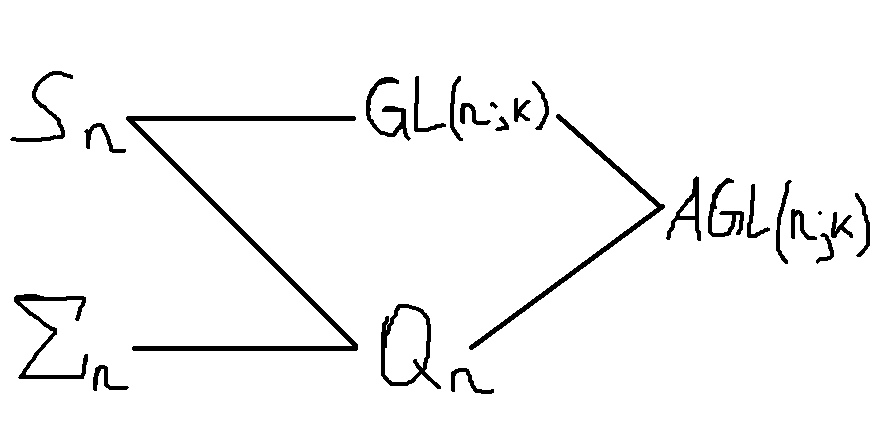
\includegraphics[scale=0.35]{dig}\\
$\sum_n; Q_n; AGL(n;k) $ - транзитивны $\Rightarrow$ инвариантны относительно них только const.\\\\
Орбитами группы $S_n$ являются множества векторов одинакового веса. Число функций одинакового веса инвариантных относительно$ S_n$ ровно $k^\frac {k+n-1}{k-1}$.\\


\thr
Орбитами группы $GL(n;k)$ являются все множества $M_\alpha=\{(a_1;\dots;a_n)\in \Omega_k^n|НОД(a_1;\dots;a_n;k)=d\}, где d|k$.\\
                   
\conseq
Число функций $n$-значной логики (от $n$-переменных ), инвариантных относительно $GL(n;k)$ равно $k^{\nu(k)},где \nu(k)$-число делителей $k$.\\


\thr
Пусть $T_k(n)$-множество всех функций $k$-значной логики с тривиальной группой инерции в $AGL(n;k)$. Тогда $$  \lim_{n\to\infty} \frac{|T_n(k)|}{|F_k(n)|}  =1$$.\\

\proof
1)Оценим сверху число неподвижных точек нетождественного фаинного преобразования $g \in AGL(n;k)$.  Рассмотрим уравнение $g(\vec{x})=\vec{x}A+\alpha;\alpha \in Z_k^n;$ $A$-невырожденная матрица над $Z_k;$ В матричном виде уравнение перепишется следующим образом:\\
$\vec{x}(E-A)=\alpha. $\\
Если $A=E$ ,то $\nexists$ решений, так как $\vec{\alpha}\neq \vec{0}$ ($g$ - нетождественное преобразование). Пусть $ C=(C_ij)_{n \times n} = E-A \neq 0 $.\\

Не ограниченная общность $c_{11} \neq 0 $ , тогда $ c_{11} x_1 + \ldots + c_{n1} x_n = a_1 $ -следствие системы, если зафиксировать $x_2;\dots;x_n $ произвольными значениями из $Z_k $, то полученное уравнение будет иметь не более $НОД(C_n;k) $ решений, а так как $C_{11} \neq 0$, то число решений при произвольной фиксации $x_2;\dots;x_n \leqslant \frac{k}{2} \rightarrow $ для всего уравнения имеем $ (\frac {k}{2})^n$. ( то есть число решений $\vec{x}(E-A) = \alpha $, не превосходит $(\frac {k}{2})^n \leqslant \frac {k^n}{2} $.)\\
2)Поскольку количество точек (неподвижных) афинной подстановки ( $ k^{l(g)} $, где $l(g)$-число циклов ) не превосзодят $\frac {k^n}{2} $, то количество независимых циклов в её разложении может превосходить $\frac {3k^n}{4} $. ( $\frac {k^n}{2} $ - циклов длины 1; $\frac {k^n}{4} $ - циклов длины 2)\\
$\rightarrow $ количество функций инвариантных относительно фиксированных подстановок $g$ не провосходят $k^{\frac{3k^n}{4}}$, так как функция должна принимать одинаковые значения на элементах каждой орбиты. \\
3) $$|AGL(n;k)| \leqslant k^{n^2+n} \rightarrow k^{\frac{3k^n}{4} +n^2 +n} \rightarrow \lim_{n\to\infty} \frac{|T_n(k)|}{|F_k(n)|} = \frac {k^{k^n}-k^{\frac {3k^n}{n}+n^2+n}}{k^{k^n}}=1$$\\

Классы эквивалентности по $\stackrel{G}{\sim}$ назовем $G$-типом. Для осуществления полной классификации необходимо построить список представителей $G$ типов.
$f^{(1)};\dots; f^{l(G)}; l(g)$- число $G$-типов.
Строится последовательность $f_1;f_2;\dots $. Среди них могу быть одинаковые представители из какого-то класса. Полагаем $ f^{(1)}=f_1$ и считаем:\\ 
$|I_G^{f(1)}|$, проверяем $f_2 \in I_G^{f(1)}$; если нет, то считаем:\\
$|I_G^{f(2)}|, при f^{(2)} =f_2$ и так далее $\dots$\\
Останавливаемся, когда :\\
$$ \sum_{i=1}^{f(G)} \frac{|G|}{|I_G^{f(i)}|} = k^{k^n} $$\\ то есть необходимость вычисления порядка групп инерции. Значение параметра $f(G)$ упрощает метод. Задача поиска этого параметра носит название задачи перечисления $G$ - типов.\\

\subsection{Инварианты, нахождение групп инерции и проверка экваивалентности.}

\opr 
Отображение $\varphi$ - называется инвариантом группы $G$, если для любого $g \in G$ и произвольной $m \in M$ справедливо равенство:\\
$\varphi(g(m))=\varphi(m)$.\\
Инвариант $\varphi$ называется полным, если из $\varphi (m_1) = \varphi(m_2) \rightarrow $ что элементы $m_1 $ и $m_2$ лежат на одной орбите группы $G$. Принимая во внимание факт, что для $G$, действующей на $F_k(n)$, орбита будет являться $G$ - типом, сформируем правило проверки эквивалентности $f_1 $ и $f_2 \in F_k(n)$.\\
Пусть $\varphi$ - инвариант группы $G$, действующей на $F_k(n)$, если $\varphi$ -полный, то $\varphi(f_1)=\varphi(f_2) $ равносильно тому, что $f_1 \stackrel{G}{\sim} f_2$;\\
Если $\varphi$неполный инвариант, то $\varphi(f_1)=\varphi(f_2) $- только необходимое условие эквивалентности. В случае, когда равенство выполнено, надо проверять другие инваринты:\\

$\sqsupset k = ?$\\
1)Для $AGL(n;k); S_n; \sum_n; Q_n $ инварианты -вес, степени нелинейности.
2)$Q_n$ - число простых импликант, число существующих переменных.
3)$S_n$ - число одночленов в многочлене Жегалкина.\\


\example 
Пусть $f(x_1;x_2;x_3)=x_1\oplus x_2$\\
$f_2(x_1;x_2;x_3)=x_1 \oplus x_2 \oplus x_3$ \\
Они не эквивалентны относительно $S_n;Q_n$, но
$f_2(x_1;x_2;x_3)=f_1((x_1;x_2;x_3)A)$\\



$A=
\begin{pmatrix}
  1 & 0 & 0\\
  0 & 1 & 0\\
  1 & 0 & 1
  
  
\end{pmatrix}$\\

$x_1 \oplus x_2;x_1;x_3$.\\


\thr
Для любого натурального $ m \geqslant 2$ и произвольной группы $G$:
$|G|=m, \exists n ,f\in f_2(n)$\\
$I_{S_n}(f) \cong G$

 







